%%%%%%%%%%%%%%%%%%%%%%
%
%   Work related to the verification of the datasets
%
%%%%%%%%%%%%%%%%%%%%%%

\section{Slices of Datacubes}

  \begin{figure}
    \centering
    \includeimage[width=\linewidth]{cube_slices_seed}
    \caption{Slice 0}
  \end{figure}

\section{Powerspectra from Simulations}

  \begin{figure}
      \centering
      % 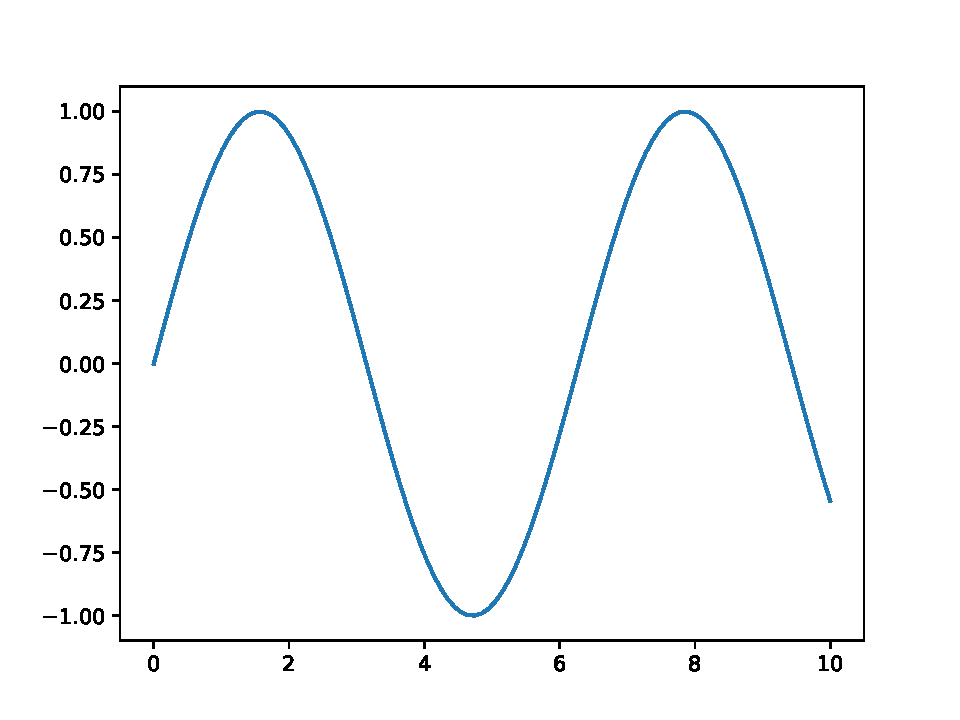
\includegraphics[width=\linewidth]{main/test.pdf}
      \includeimage[width=\linewidth]{average_matter_power_spectra}
      \caption{Average matter power spectra at different redshifts.}
    \end{figure}

    \begin{figure}
      \centering
      % 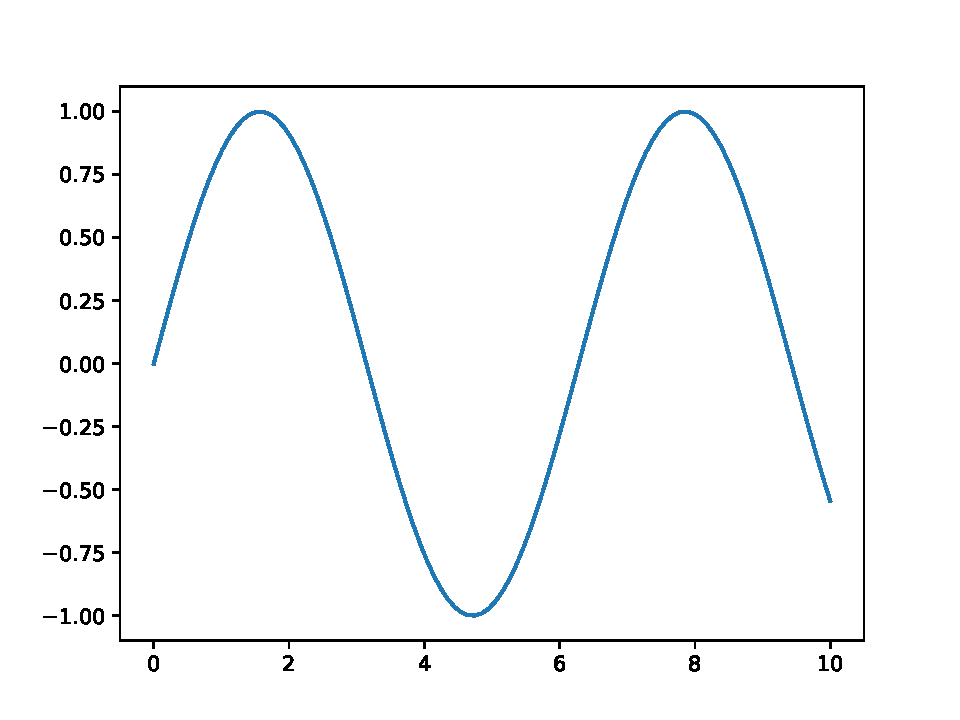
\includegraphics[width=\linewidth]{main/test.pdf}
      \includeimage[width=\linewidth]{average_potential_power_spectra}
      \caption{Average potential power spectra at different redshifts.}
    \end{figure}

\section{Powerspectra from Datacubes}

\section{Analytical Bispectra}

  \begin{figure}
    \centering
    \label{fig:data:verification:bispectrum_angles}
    \begin{tikzpicture}
    \colorlet{veccol}{green!70!black}
    \colorlet{vcol}{green!70!black}
    \colorlet{xcol}{blue!85!black}
    \colorlet{projcol}{xcol!60}
    \colorlet{unitcol}{xcol!60!black!85}
    \colorlet{myblue}{blue!70!black}
    \colorlet{myred}{red!90!black}
    \colorlet{mypurple}{blue!50!red!80!black!80}
    \tikzstyle{vector}=[->,very thick,xcol]
  
  
    % Define the k vector
    \def\Kone{5}
    \def\Ktwo{5}
    \def\Kthree{5}
    \def\staplelength{1}
    \def\anglealpha{60}
    \def\anglebeta{60}
    \def\anglegamma{60}
  
    \coordinate (k1start) at (0,0);
    \coordinate (k2start) at (\anglegamma:\Kone);
    \coordinate (k3start) at (\Kthree,0);
  
    % \Draw vector
    \draw[vector] (k1start) -- (k2start) node[midway, left=20, above=5, right=0] {$\vb{k}_1$};
    \draw[vector] (k2start) -- (k3start) node[midway, right=20, above=5, left=0] {$\vb{k}_2$};
    \draw[vector] (k3start) -- (k1start) node[midway, below=5] {$\vb{k}_3$};
    
    
    % coordinates for the extra stapled lines
    \coordinate (k1staplestop) at ({\Kone*cos(\anglegamma)+\staplelength*cos(\anglegamma)}, {\Kone*sin(\anglegamma)+\staplelength*sin(\anglegamma)});
    \coordinate (k2staplestop) at ({\Kthree+\staplelength*cos(\anglebeta)}, {-\staplelength*sin(\anglebeta)});
    \coordinate (k3staplestop) at ({-\staplelength}, 0);
  
    \draw[dashed] (k2start) -- (k1staplestop);
    \draw[dashed] (k3start) -- (k2staplestop);
    \draw[dashed] (k1start) -- (k3staplestop);
  
    \draw pic[-, thick, "$\alpha$", draw=black, angle radius = 25, angle eccentricity=1.3]{angle = k1start--k2start--k3start};
    \draw pic[-, thick, "$\beta$", draw=black, angle radius = 25, angle eccentricity=1.3]{angle = k2start--k3start--k1start};
    \draw pic[-, thick, "$\gamma$", draw=black, angle radius = 25, angle eccentricity=1.3]{angle = k3start--k1start--k2start};
  
    \draw pic[-, thick, "$\theta_{12}$", draw=black, angle radius = 15, angle eccentricity=1.6]{angle = k3start--k2start--k1staplestop};
    \draw pic[-, thick, "$\theta_{23}$", draw=black, angle radius = 15, angle eccentricity=1.6]{angle = k1start--k3start--k2staplestop};
    \draw pic[-, thick, "$\theta_{31}$", draw=black, angle radius = 15, angle eccentricity=1.6]{angle = k2start--k1start--k3staplestop};
  \end{tikzpicture}
    \caption{Angles in arbitrary bispectrum triangle configuration.}
  \end{figure}
  \begin{equation}
    B^{(3)}(k_1,k_2,k_3) = 2\mathcal{P}(k_1)\mathcal{P}(k_2)F_2(\vec{k}_1, \vec{k}_2) + \mathrm{cyc}
  \end{equation}

  \begin{equation}
    F_2(\vec{k}_1,\vec{k}_2) = \frac{5}{7} + \frac{x}{2}\left(\frac{k_1}{k_2}+\frac{k_2}{k_1}\right) + \frac{2}{7}x^2,
  \end{equation}
  where $x = \hat{\vec{k}}_1 \cdot \hat{\vec{k}}_2 = \cos{\theta_{12}}$, where $\theta_{12}$ is the angle spanned by $\vec{k}_1$ and $\vec{k}_2$. We could thus consequently write: $F_2(\vec{k}_1,\vec{k_2}) = F_2(k_1,k_2,\theta_{12})$

  Given $k_1$ and $k_2$ and $\theta_{12}$ we have the following relations, with reference to \cref{fig:data:verification:bispectrum_angles}:


  \begin{equation}
    \begin{split}
      \alpha &= \pi-\theta_{12}\\
      \beta &= \pi-\theta_{23}\\
      \gamma &= \pi-\theta_{31}
    \end{split}
  \end{equation} 

  From cosine rule:
  \begin{equation}
    k_3 = \sqrt{k_1^2 + k_2^2 - 2k_1k_2\cos\alpha}
  \end{equation}

  From the rule of sines \TODO{explain more?}:
  \begin{equation}
    \begin{split}
      \beta &= \arcsin\left(\frac{k_1}{k_3}\sin\alpha\right)\\
      \gamma &= \arcsin\left(\frac{k_2}{k_3}\sin\alpha\right)
    \end{split}
  \end{equation}

  \begin{figure}
    \centering
    \includeimage[width=\linewidth]{analytical_bispectra}
  \end{figure}

\section{Bispectra from Cube}
  \subsection{Binning}
    % \begin{equation}
    %   k_\mathrm{new
    % \end{equation}

    \begin{figure}
      \centering
      \includeimage[width=\linewidth]{binning_example}
    \end{figure}

  \subsection{Bispectra}
    \begin{figure}
      \centering
      \includeimage[width=\linewidth]{average_bispectra}
    \end{figure}


